% Generated by tools/manuscript/build.py from docs/dispersion-model.md and
% docs/repeat-runs-pilot.md. Edit those pages and rebuild; do not edit this file.
% Options for packages loaded elsewhere
\PassOptionsToPackage{unicode}{hyperref}
\PassOptionsToPackage{hyphens}{url}
\documentclass[
  11pt,
  a4paper,
]{article}
\usepackage{xcolor}
\usepackage[margin=2.6cm]{geometry}
\usepackage{amsmath,amssymb}
\setcounter{secnumdepth}{5}
\usepackage{iftex}
\ifPDFTeX
  \usepackage[T1]{fontenc}
  \usepackage[utf8]{inputenc}
  \usepackage{textcomp} % provide euro and other symbols
\else % if luatex or xetex
  \usepackage{unicode-math} % this also loads fontspec
  \defaultfontfeatures{Scale=MatchLowercase}
  \defaultfontfeatures[\rmfamily]{Ligatures=TeX,Scale=1}
\fi
\usepackage{lmodern}
\ifPDFTeX\else
  % xetex/luatex font selection
\fi
% Use upquote if available, for straight quotes in verbatim environments
\IfFileExists{upquote.sty}{\usepackage{upquote}}{}
\IfFileExists{microtype.sty}{% use microtype if available
  \usepackage[]{microtype}
  \UseMicrotypeSet[protrusion]{basicmath} % disable protrusion for tt fonts
}{}
\usepackage{setspace}
\makeatletter
\@ifundefined{KOMAClassName}{% if non-KOMA class
  \IfFileExists{parskip.sty}{%
    \usepackage{parskip}
  }{% else
    \setlength{\parindent}{0pt}
    \setlength{\parskip}{6pt plus 2pt minus 1pt}}
}{% if KOMA class
  \KOMAoptions{parskip=half}}
\makeatother
\usepackage{longtable,booktabs,array}
\usepackage{caption}
\captionsetup[table]{skip=6pt}
\newcounter{none} % for unnumbered tables
\usepackage{calc} % for calculating minipage widths
% Correct order of tables after \paragraph or \subparagraph
\usepackage{etoolbox}
\makeatletter
\patchcmd\longtable{\par}{\if@noskipsec\mbox{}\fi\par}{}{}
\makeatother
% Allow footnotes in longtable head/foot
\IfFileExists{footnotehyper.sty}{\usepackage{footnotehyper}}{\usepackage{footnote}}
\makesavenoteenv{longtable}
\setlength{\emergencystretch}{3em} % prevent overfull lines
\providecommand{\tightlist}{%
  \setlength{\itemsep}{0pt}\setlength{\parskip}{0pt}}
\usepackage{bookmark}
\IfFileExists{xurl.sty}{\usepackage{xurl}}{} % add URL line breaks if available
\urlstyle{same}
% fallback for those not using the hyperref driver hyperxmp:
\makeatletter
\@ifundefined{xmpquote}{\newcommand{\xmpquote}[1]{#1}}{}
\makeatother
\hypersetup{
  pdftitle={A per-paper dispersion model},
  pdfauthor={ReplicHAI Workgroup},
  hidelinks,
  pdfcreator={LaTeX via pandoc}}

\title{A per-paper dispersion model}
\author{ReplicHAI Workgroup\\[3pt]
{\normalsize Latere AI}\\[1pt]
{\normalsize\href{https://replichai.latere.ai}{replichai.latere.ai}}}
\date{9 October 2026}

\usepackage{needspace}
\usepackage{caption}
\usepackage{tikz}
\usetikzlibrary{positioning,calc,arrows.meta,shapes.geometric}
\usepackage{draftwatermark}
\DraftwatermarkOptions{text=DRAFT, angle=45, color={[gray]{0.90}}}
\begin{document}
\maketitle

\setstretch{1.08}
When an AI agent is asked to reproduce the same paper several times, its
runs do not agree with each other. This note proposes how to measure
that disagreement and how to tell what causes it. Nothing here has been
estimated yet. It is written for review before a study is registered.

\section{Research question}\label{research-question}

\textbf{When repeat runs of one paper disagree about whether its results
reproduce, where does the disagreement come from: the paper, the
conditions the run had, or chance?}

This is not the question of whether a paper reproduces. Each run already
answers that, result by result. The question is how far that answer
depends on which run gave it. The two come apart: a paper whose results
fail in every run shows no disagreement at all, exactly like a paper
whose results reproduce in every run. Disagreement is largest when a
result reproduces in about half of the runs.

Three questions make that precise:

\begin{enumerate}
\def\labelenumi{\arabic{enumi}.}
\tightlist
\item
  \textbf{How large is it?} For each result a paper reports, how likely
  is it that two independent runs disagree about whether it reproduced?
\item
  \textbf{What does it belong to?} How much of the disagreement comes
  from the paper and the materials its authors released, how much from
  the environment of the run (which AI agent ran it, what it could reach
  on the network, which copy of the paper it was given), and how much is
  left as chance between runs under the same conditions?
\item
  \textbf{Is it a property of the paper?} Does the amount of
  disagreement differ reliably from paper to paper, does the ranking of
  papers hold when the environment changes, and does disagreement rise
  on exactly the results affected when a stated detail is withheld from
  a paper?
\end{enumerate}

The answer to the first question, averaged over a paper's results, is
the paper's disagreement. It is written \(H\) below: the chance that two
runs disagree about one result of the paper. It is 0 when every run
agrees on every result, and at most 0.5, when each result reproduces in
half of the runs.

A low \(H\) says a run's outcome is repeatable. It does not say the
outcome is right: every run can agree and be wrong, for instance when
all of them are refused the same page or make the same mistake. Whether
outcomes are right is a separate question, answered by comparing them
with outcomes people verified by hand, which the intended corpus has.
Repeatability comes first, because an outcome that changes from run to
run cannot be checked against anything.

The answer to the third question decides what an audit may report. If it
is yes, \(H\) can be reported as a measure of how completely the paper
and its materials pin down its own analysis. If not, the disagreement
describes the auditing instrument, and a single run's verdict has to be
reported as one draw under stated conditions.

The estimands and the model-free estimator below answer the first
question, the model the second, and the three tests the third. The study
in one picture:

\par\nobreak\addvspace{\medskipamount}\noindent\begin{minipage}{\linewidth}\centering
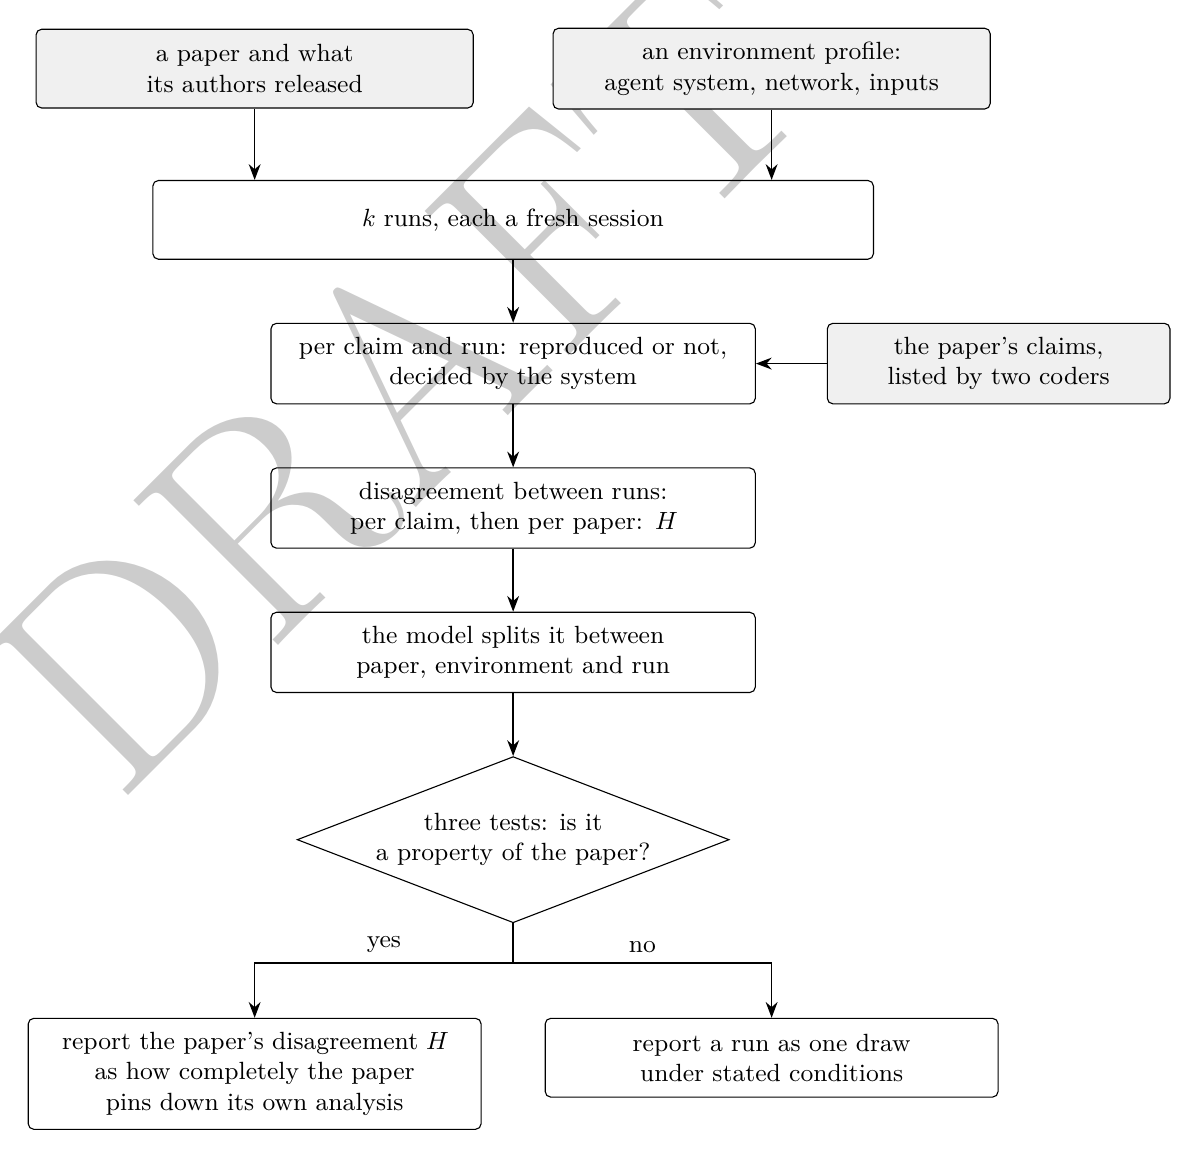
\begin{tikzpicture}[
  font=\small, >=Stealth,
  box/.style={draw, rounded corners=2pt, align=center, inner sep=5pt, minimum height=10mm, text width=#1},
  box/.default=52mm,
  given/.style={box=#1, fill=black!6},
  given/.default=52mm,
  flow/.style={->, semithick},
]
  \node[given] (paper) {a paper and what\\its authors released};
  \node[given, right=10mm of paper] (env) {an environment profile:\\agent system, network, inputs};
  \node[box=88mm, below=9mm of $(paper.south)!0.5!(env.south)$] (runs) {$k$ runs, each a fresh session};
  \node[box=58mm, below=8mm of runs] (y) {per claim and run: reproduced or not,\\decided by the system};
  \node[given=40mm, right=9mm of y] (claims) {the paper's claims,\\listed by two coders};
  \node[box=58mm, below=8mm of y] (h) {disagreement between runs:\\per claim, then per paper: $H$};
  \node[box=58mm, below=8mm of h] (model) {the model splits it between\\paper, environment and run};
  \node[draw, diamond, aspect=2.6, align=center, inner sep=1pt, below=8mm of model] (test) {three tests: is it\\a property of the paper?};
  \coordinate (split) at ($(test.south)+(0,-5mm)$);
  \node[box=54mm, anchor=north east] (yes) at ($(split)+(-4mm,-7mm)$) {report the paper's disagreement $H$\\as how completely the paper\\pins down its own analysis};
  \node[box=54mm, anchor=north west] (no) at ($(split)+(4mm,-7mm)$) {report a run as one draw\\under stated conditions};

  \draw[flow] (paper.south) -- (runs.north -| paper.south);
  \draw[flow] (env.south) -- (runs.north -| env.south);
  \draw[flow] (runs) -- (y);
  \draw[flow] (claims) -- (y);
  \draw[flow] (y) -- (h);
  \draw[flow] (h) -- (model);
  \draw[flow] (model) -- (test);
  \draw[semithick] (test.south) -- (split);
  \draw[flow] (split) -| node[pos=0.25, above] {yes} (yes.north);
  \draw[flow] (split) -| node[pos=0.25, above] {no} (no.north);
\end{tikzpicture}
\captionof{figure}{The study in one picture. $H$ is the chance that two runs disagree about one result of the paper, averaged over its results. The shaded boxes are fixed before any run.}
\end{minipage}\par\addvspace{\medskipamount}

The evidence that prompted the question is a pilot of 49 runs of three
papers (Appendix A): the spread between runs is real and large, and most
of it in the pilot came from the agent system, the network and labeling
rather than the paper. The model therefore treats the environment as a
facet to estimate, not as noise, and gives each paper its own dispersion
instead of pooling one.

\section{Setting}\label{setting}

ReplicHAI audits the reproducibility of a research paper with a coding
agent. Given a paper, one \textbf{run} finds what the authors released
and splits the paper into components. It places each component in the
inner loop, the part a machine can re-run (the analysis, the model or
the pipeline), or in the outer loop, the study with human participants,
which is never re-run or simulated. It re-runs the inner loop, marks
each inner component verified, partial or blocked, records where its
numbers disagree with the paper's, and lists the hidden decisions:
choices a reimplementation has to make that the paper does not state. A
second stage grades the run against a fixed rubric, and a run that falls
short is revised.

Three things can differ between two runs of one paper, and the model
keeps them apart:

\begin{itemize}
\tightlist
\item
  the \textbf{paper}, with the materials its authors released;
\item
  the \textbf{environment} of the run: the agent system (the coding
  agent and the model behind it), the network it may reach, and the copy
  of the paper and of the artifacts it was given;
\item
  the \textbf{run} itself: a fresh session of the same agent on the same
  inputs does not make the same choices twice.
\end{itemize}

A \textbf{claim} is one quantitative result the paper reports, such as a
test statistic, an estimate or a count. Whether a run reproduced a claim
is the unit the model is built on.

\section{Why not plain generalizability
theory}\label{why-not-plain-generalizability-theory}

A generalizability study over paper × prompt × run, where the prompt is
the instructions the agent is given and runs are nested in each paper
and prompt cell, estimates one run variance component for the whole
corpus, \(\sigma^2_{r:pq}\), and treats it as error around each paper's
mean. That is the right tool for asking how reliably a paper's
\emph{mean} outcome is measured. It cannot say that one paper's runs
disagree more than another's, because it assumes they all disagree by
the same amount. The question here is the opposite one, so the run
variance has to be allowed to differ by paper and to be modeled in its
own right.

\section{Data and notation}\label{data-and-notation}

{\def\LTcaptype{none} % do not increment counter
\par\nobreak\addvspace{\medskipamount}\noindent\begin{minipage}{\linewidth}
\begin{tabular}{@{}
  >{\raggedright\arraybackslash}p{(\linewidth - 2\tabcolsep) * \real{0.1667}}
  >{\raggedright\arraybackslash}p{(\linewidth - 2\tabcolsep) * \real{0.8333}}@{}}
\toprule\noalign{}
\begin{minipage}[b]{\linewidth}\raggedright
Symbol
\end{minipage} & \begin{minipage}[b]{\linewidth}\raggedright
Meaning
\end{minipage} \\
\midrule\noalign{}
\(p = 1, \dots, P\) & papers \\
\(c = 1, \dots, m_p\) & claims of paper \(p\): the paper's reported
quantitative results, frozen per paper by two human coders before any
run is scored \\
\(e = 1, \dots, E\) & environment profiles: the agent system and model,
the network policy, the copy of the paper, the artifact snapshot. A
small number of designed levels, crossed with papers \\
\(r = 1, \dots, k\) & runs, nested in paper × profile \\
\(Y_{pcer} \in \{0, 1\}\) & whether claim \(c\) reproduced in run \(r\):
the run's observed value is within the registered tolerance of the
reported value, decided by the system from the run's reported number,
never by the agent's label \\
\bottomrule\noalign{}
\end{tabular}
\end{minipage}\par\addvspace{\medskipamount}
}

A claim the run did not attempt, or could not run, is \(Y = 0\) and also
carries a cause (environment, paper, artifacts) recorded by the run, so
a blocked claim can be analyzed by why it was blocked.

\section{Estimands}\label{estimands}

\textbf{Reproduction probability of a claim.}
\(q_{pce} = \Pr(Y_{pcer} = 1)\) for a fresh run under profile \(e\).

\textbf{Claim instability.} The probability that two independent runs
disagree about claim \(c\):
\begin{equation}
h_{pce} = 2\, q_{pce}\,(1 - q_{pce}).
\end{equation}

It is zero for a claim that always or never reproduces, and largest at
\(q = 1/2\).

\textbf{Paper instability.} The paper's disagreement \(H\) from the
research question, the average over the paper's claims:
\begin{equation}
H_{pe} = \frac{1}{m_p} \sum_{c=1}^{m_p} h_{pce}.
\end{equation}

This is the primary per-paper dispersion: the chance that two runs
disagree about a claim of this paper, under this environment. It has a
plain reading and a direct estimator, and it does not depend on how an
agent decomposes the paper, because the claims are frozen.

\textbf{Run-shared dispersion.} How much a whole run moves together: a
run that cannot reach the paper, or loses its dependencies, fails many
claims at once. This is \(s_{pe}\) in the model below.

\textbf{Environment effects.} The shift in reproduction, \(\beta_e\),
and in run-shared dispersion, \(\alpha_e\), between profiles, and the
paper × environment interaction \(v_{pe}\): whether the environment
changes \emph{which} papers reproduce.

\section{A model-free estimator}\label{a-model-free-estimator}

With \(k \ge 2\) runs and \(x_{pce}\) successes on claim \(c\),
\begin{equation}
\hat h_{pce} = \frac{2\, x_{pce}\,(k - x_{pce})}{k\,(k - 1)}
\end{equation}
is unbiased for \(h_{pce}\), and \(\hat H_{pe}\) is the mean of
\(\hat h_{pce}\) over claims. Because the claims of a paper act as
replicates, it is far more precise at a small \(k\) than a run-level
standard deviation. In a simulation with 15 claims, a third of them
unstable (\(q = 0.5\)) and the rest stable (\(q = 0.95\)), the 95\%
range of \(\hat H / H\) was:

{\def\LTcaptype{none} % do not increment counter
\par\nobreak\addvspace{\medskipamount}\noindent\begin{minipage}{\linewidth}
\begin{tabular}{@{}
  >{\raggedright\arraybackslash}p{(\linewidth - 6\tabcolsep) * \real{0.2432}}
  >{\raggedright\arraybackslash}p{(\linewidth - 6\tabcolsep) * \real{0.2973}}
  >{\raggedright\arraybackslash}p{(\linewidth - 6\tabcolsep) * \real{0.1351}}
  >{\raggedright\arraybackslash}p{(\linewidth - 6\tabcolsep) * \real{0.3243}}@{}}
\toprule\noalign{}
\begin{minipage}[b]{\linewidth}\raggedright
Runs per paper \(k\)
\end{minipage} & \begin{minipage}[b]{\linewidth}\raggedright
95\% range of \(\hat H / H\)
\end{minipage} & \begin{minipage}[b]{\linewidth}\raggedright
Spread
\end{minipage} & \begin{minipage}[b]{\linewidth}\raggedright
Run-level SD, same data
\end{minipage} \\
\midrule\noalign{}
3 & 0.39 to 1.55 & 4.0× & can be 0; unusable \\
5 & 0.64 to 1.39 & 2.2× & 0.34 to 1.65 \\
8 & 0.73 to 1.29 & 1.8× & 0.49 to 1.51 \\
10 & 0.77 to 1.26 & 1.6× & 0.54 to 1.44 \\
\bottomrule\noalign{}
\end{tabular}
\end{minipage}\par\addvspace{\medskipamount}
}

For comparison, the 95\% interval on a single paper's run standard
deviation from \(k\) normal draws is \(0.52\) to \(6.28\) times the
estimate at \(k = 3\), \(0.60\) to \(2.87\) at \(k = 5\), and \(0.69\)
to \(1.83\) at \(k = 10\).

\section{The model}\label{the-model}

A claim-level logistic mixed model in which each paper has its own
run-shared variance:
\begin{gather}
\operatorname{logit} \Pr(Y_{pcer} = 1) = \beta_0 + \beta_e + u_p + v_{pe} + w_{pc} + \eta_{per} \\
u_p \sim N(0, \tau_u^2), \qquad v_{pe} \sim N(0, \tau_v^2), \qquad w_{pc} \sim N(0, \tau_w^2) \\
\eta_{per} \sim N\!\left(0,\, s_{pe}^2\right), \qquad \log s_{pe} = \alpha_0 + \alpha_e + \omega_p, \qquad \omega_p \sim N(0, \tau_\omega^2) \\
\operatorname{corr}(u_p, \omega_p) = \rho.
\end{gather}

\begin{itemize}
\tightlist
\item
  \(u_p\) is how reproducible the paper is overall; \(w_{pc}\) how hard
  each claim is.
\item
  \(\eta_{per}\) is the run's shared shock: everything that moves all of
  a run's claims together. Its standard deviation \(s_{pe}\) belongs to
  the paper and the environment, which is the formal version of ``each
  paper has its own dispersion''.
\item
  Claim-specific disagreement between runs, beyond the shared shock, is
  the Bernoulli variation of claims whose \(q\) is away from 0 and 1.
  That is where a decision the paper left open shows up: it moves one
  claim, not the whole run.
\end{itemize}

The same model as a picture. Each box on the left moves the chance that
a claim reproduces. The box at the bottom sets how large a run's shock
is, and it is where a paper gets a dispersion of its own:

\par\nobreak\addvspace{\medskipamount}\noindent\begin{minipage}{\linewidth}\centering
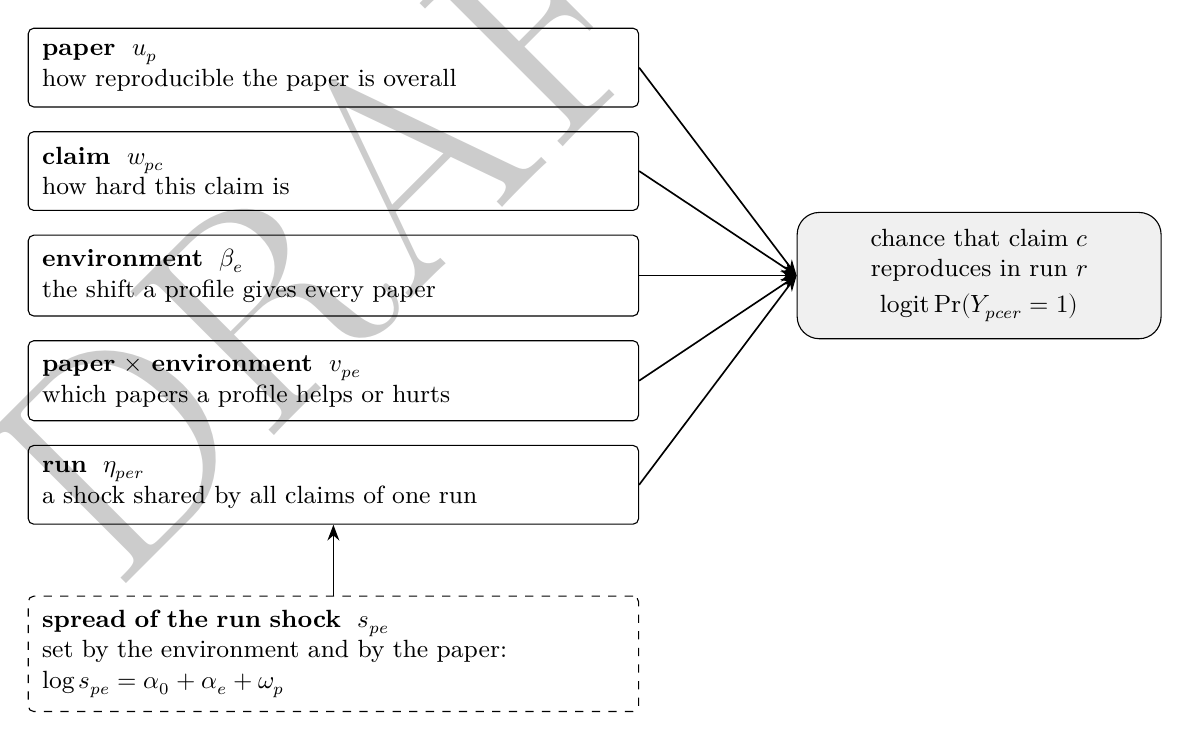
\begin{tikzpicture}[
  font=\small, >=Stealth,
  box/.style={draw, rounded corners=2pt, align=left, inner sep=5pt, minimum height=10mm, text width=#1},
  box/.default=74mm,
  flow/.style={->, semithick},
]
  \node[box] (u) {\textbf{paper} \ $u_p$\\how reproducible the paper is overall};
  \node[box, below=3mm of u] (w) {\textbf{claim} \ $w_{pc}$\\how hard this claim is};
  \node[box, below=3mm of w] (b) {\textbf{environment} \ $\beta_e$\\the shift a profile gives every paper};
  \node[box, below=3mm of b] (v) {\textbf{paper $\times$ environment} \ $v_{pe}$\\which papers a profile helps or hurts};
  \node[box, below=3mm of v] (eta) {\textbf{run} \ $\eta_{per}$\\a shock shared by all claims of one run};
  \node[box, dashed, below=9mm of eta] (s) {\textbf{spread of the run shock} \ $s_{pe}$\\set by the environment and by the paper:\\\mbox{$\log s_{pe}=\alpha_0+\alpha_e+\omega_p$}};

  \node[draw, rounded corners=8pt, fill=black!6, align=center, inner sep=6pt, text width=42mm, right=20mm of b] (y)
    {chance that claim $c$\\reproduces in run $r$\\[2pt]\mbox{$\operatorname{logit}\Pr(Y_{pcer}=1)$}};

  \foreach \source in {u, w, b, v, eta} \draw[flow] (\source.east) -- (y.west);
  \draw[flow] (s) -- (eta);
\end{tikzpicture}
\captionof{figure}{What moves a claim's outcome in the model. The dashed box is where a paper gets a dispersion of its own: $\omega_p$ is what the third research question asks about.}
\end{minipage}\par\addvspace{\medskipamount}

The split between the two is the one the pilot points at. On the latent
scale, the share of a claim's between-run variance that is shared by the
whole run is
\begin{equation}
\lambda_{pe} = \frac{s_{pe}^2}{s_{pe}^2 + \pi^2/3}.
\end{equation}

A high \(\lambda\) says the runs differ as wholes: the environment, or
the agent's trajectory. A low \(\lambda\) with a high \(H\) says
individual claims flip independently: what the paper did not specify.

If a continuous run score is preferred to claim outcomes, the same idea
is a location-scale model on the score \(S_{per}\) (for example the
logit of the share of claims reproduced):
\begin{equation}
S_{per} = \beta_0 + \beta_e + u_p + v_{pe} + \varepsilon_{per}, \qquad \varepsilon_{per} \sim N(0, \sigma_{pe}^2), \qquad \log \sigma_{pe} = \alpha_0 + \alpha_e + \omega_p.
\end{equation}

That version fits in brms as

\begin{verbatim}
bf(S ~ env + (1|i|paper) + (1|paper:env),
   sigma ~ env + (1|i|paper))
\end{verbatim}

The claim-level version needs a short Stan program, because the run
effect's standard deviation is itself hierarchical across papers. Both
are fit on all runs at once, which handles unequal numbers of runs and
claims.

\section{Is dispersion a property of the
paper?}\label{is-dispersion-a-property-of-the-paper}

Three tests, registered before any outcome is seen. All three have to
pass for the study to say that dispersion describes the paper.

\begin{enumerate}
\def\labelenumi{\arabic{enumi}.}
\tightlist
\item
  \textbf{Between-paper variance of dispersion is above zero.}
  \(\tau_\omega^2 > 0\) in the model, by a likelihood-ratio test against
  the model without \(\omega_p\) (the null is on the boundary, so the
  reference distribution is a 50:50 mixture of \(\chi^2_0\) and
  \(\chi^2_1\)), or by its posterior. For the model-free estimator, the
  between-paper variance of \(\hat H_p\) must exceed the mean of its
  within-paper sampling variance, estimated by resampling runs.
\item
  \textbf{The ranking survives a change of environment.} Papers ranked
  by \(H\) under two agent systems must agree (Spearman correlation
  registered in advance). A property of the paper does not reorder when
  the agent changes. The pilot already fails this on four of six crude
  measures, with too few runs to decide.
\item
  \textbf{Dispersion follows what was withheld.} Take papers whose
  analysis is fully specified. Run them as published, then with one
  stated detail removed (a seed, a degrees-of-freedom method, an
  exclusion rule). The claims that detail affects must gain instability
  and the others must not. The unedited papers also give the
  instrument's noise floor: their \(H\) is what the agent and
  environment contribute alone.
\end{enumerate}

\section{Reliability}\label{reliability}

For ranking papers by reproduction level, the generalizability
coefficient with paper as the object of measurement is
\begin{equation}
E\rho^2 = \frac{\tau_u^2}{\tau_u^2 + \tau_v^2 / n_e + \sigma^2_{\text{res}} / (n_e\, k)}.
\end{equation}

For dispersion, the reliability of \(\hat H_p\) is the share of its
variance across papers that is not sampling noise. Estimate it by
splitting each paper's runs into halves, correlating \(\hat H_p\) across
papers between the halves, and applying the Spearman-Brown correction.
Require at least 0.8 before reporting a single paper's dispersion.

A criterion proposed earlier in this project, ``if prompt-level variance
exceeds run-level variance we do not have an instrument'', compares two
error terms. A prompt's main effect moves every paper equally and does
not change a ranking; what matters is the paper × prompt interaction
relative to \(\tau_u^2\), which \(E\rho^2\) already contains. Three
prompts give two degrees of freedom for a prompt main effect, so prompts
are a fixed facet, and no claim generalizes beyond the prompts tested.

\Needspace{24\baselineskip}
\section{Sample size}\label{sample-size}

The intended corpus is the 76 CHI papers that have shared both data and
code, whose reproduction outcomes were verified by hand (Iarygina,
Hornbæk and Mottelson, 2026). That caps the corpus at 76 papers, so runs
per paper is the lever that is left. Pooled components are well
estimated at \(k = 3\); per-paper dispersion is not. A design that can
grow into the main study:

{\def\LTcaptype{none} % do not increment counter
\par\nobreak\addvspace{\medskipamount}\noindent\begin{minipage}{\linewidth}
\begin{tabular}{@{}
  >{\raggedright\arraybackslash}p{(\linewidth - 4\tabcolsep) * \real{0.2200}}
  >{\raggedright\arraybackslash}p{(\linewidth - 4\tabcolsep) * \real{0.3800}}
  >{\raggedright\arraybackslash}p{(\linewidth - 4\tabcolsep) * \real{0.4000}}@{}}
\toprule\noalign{}
\begin{minipage}[b]{\linewidth}\raggedright
Stage
\end{minipage} & \begin{minipage}[b]{\linewidth}\raggedright
Papers × runs
\end{minipage} & \begin{minipage}[b]{\linewidth}\raggedright
Purpose
\end{minipage} \\
\midrule\noalign{}
Internal pilot & 16 × 8, one profile & Estimate \(\tau_\omega^2\) and
the reliability of \(\hat H_p\). These runs count toward the main
study \\
Main study & the other 60 × 5 if \(\tau_\omega^2\) is detectable,
otherwise × 3 and no per-paper dispersion claims & Paper levels and, if
supported, dispersion \\
Environment facet & 20 × 2 more profiles × 4 & \(\beta_e\),
\(\alpha_e\), the paper × environment interaction, and test 2 \\
Noise floor and withholding & 5 to 8 fully specified papers, as
published and with one detail withheld & Test 3 \\
\bottomrule\noalign{}
\end{tabular}
\end{minipage}\par\addvspace{\medskipamount}
}

The decision rule between ``× 5'' and ``× 3'' is written into the
registration.

\section{Assumptions and open
questions}\label{assumptions-and-open-questions}

\begin{itemize}
\tightlist
\item
  Runs are independent given paper and profile. This needs fresh
  sessions with no shared cache, recorded inputs, and the analysis of
  the first graded attempt, before any revision the grader requests.
\item
  Claims are fixed by people, with agreement between two coders
  reported. Claims that are qualitative are out of scope and counted,
  not dropped.
\item
  The match tolerance is registered per claim type before runs are
  scored.
\item
  How launch failures are excluded is stated before outcomes are seen.
\item
  A run's blocker cause is recorded in a closed list, so
  environment-caused zeros can be separated from paper-caused zeros in a
  sensitivity analysis.
\end{itemize}

\section*{References}\label{references}
\addcontentsline{toc}{section}{References}

Iarygina, O., Hornbæk, K., and Mottelson, A. (2026). On the
Computational Reproducibility of Human-Computer Interaction.
\emph{Proceedings of the 2026 CHI Conference on Human Factors in
Computing Systems}, 1--16. \url{https://doi.org/10.1145/3772318.3791129}

\appendix

\section{What repeat runs of one paper
showed}\label{what-repeat-runs-of-one-paper-showed}

Three papers were audited ten to twenty-one times each on 10 and 11
September 2026, all under one method, meaning one set of instructions
and one rubric (digest \texttt{sha256:f9af95bb…}). This appendix records
what those runs show about the idea that run-to-run variation measures
what a paper left unsaid. The data was analyzed on 9 October 2026.

\textbf{The short answer:} the runs vary a lot, but most of the
variation traced so far comes from the agent system, the network, how
the agent labels its own results, and the grader's revisions. The
paper's own silence is a real part of it, and a small one. A design that
reads the spread as a property of the paper has to remove or measure
those other sources first. The main text proposes the measurement.

\subsection{The runs}\label{the-runs}

{\def\LTcaptype{none} % do not increment counter
\par\nobreak\addvspace{\medskipamount}\noindent\begin{minipage}{\linewidth}
\begin{tabular}{@{}
  >{\raggedright\arraybackslash}p{(\linewidth - 6\tabcolsep) * \real{0.5814}}
  >{\raggedright\arraybackslash}p{(\linewidth - 6\tabcolsep) * \real{0.1860}}
  >{\raggedright\arraybackslash}p{(\linewidth - 6\tabcolsep) * \real{0.1163}}
  >{\raggedright\arraybackslash}p{(\linewidth - 6\tabcolsep) * \real{0.1163}}@{}}
\toprule\noalign{}
\begin{minipage}[b]{\linewidth}\raggedright
Paper
\end{minipage} & \begin{minipage}[b]{\linewidth}\raggedright
Called below
\end{minipage} & \begin{minipage}[b]{\linewidth}\raggedright
Runs started
\end{minipage} & \begin{minipage}[b]{\linewidth}\raggedright
With a verdict
\end{minipage} \\
\midrule\noalign{}
Johnson, Sengupta, Schöning and Hecht (2016). \emph{The Geography and
Importance of Localness in Geotagged Social Media.} CHI '16, 515--526.
\href{https://doi.org/10.1145/2858036.2858122}{10.1145/2858036.2858122}
& Geography & 10 & 10 \\
Ou (2026). \emph{Progressive Autonomy as Preference Learning: A
Formalization of Trust Calibration for Agentic Tool Use.}
\href{https://arxiv.org/abs/2605.19151}{arXiv:2605.19151} & Progressive
autonomy & 18 & 6 \\
Kay, Matuszek and Munson (2015). \emph{Unequal Representation and Gender
Stereotypes in Image Search Results for Occupations.} CHI '15,
3819--3828.
\href{https://doi.org/10.1145/2702123.2702520}{10.1145/2702123.2702520}
& Unequal representation & 21 & 10 \\
\bottomrule\noalign{}
\end{tabular}
\end{minipage}\par\addvspace{\medskipamount}
}

Each run is its own private repository under \texttt{open-hai}, named
after the paper with a four-character suffix. The suffixes below refer
to those repositories.

\textbf{The runs with no verdict failed at launch.} Eight repositories
on the third paper were created within 20 seconds of each other and hold
no commits. Most of the rest hold only the system's identity commit,
written seconds after the repository was created, with no agent commit
after it. Runs started later the same day completed 16 of 16. The
completion rates in the table therefore say when each paper was run, not
how hard it is. No published record says why a run stopped, so this
reading rests on timing, not on a recorded cause.

\subsection{Two agent systems ran every
paper}\label{two-agent-systems-ran-every-paper}

Each run's \texttt{environment.json} names its harness and model. The
pilot mixed Claude Code on \texttt{claude-opus-5} with Codex on
\texttt{gpt-6-astra}, under the same method digest. The manifest the
registry reads, \texttt{replication.json}, records neither, so the mix
is invisible to anything that reads only the manifest.

{\def\LTcaptype{none} % do not increment counter
\par\nobreak\addvspace{\medskipamount}\noindent\begin{minipage}{\linewidth}
\begin{tabular}{@{}
  >{\raggedright\arraybackslash}p{(\linewidth - 12\tabcolsep) * \real{0.1905}}
  >{\raggedright\arraybackslash}p{(\linewidth - 12\tabcolsep) * \real{0.1310}}
  >{\raggedright\arraybackslash}p{(\linewidth - 12\tabcolsep) * \real{0.0714}}
  >{\raggedright\arraybackslash}p{(\linewidth - 12\tabcolsep) * \real{0.1667}}
  >{\raggedright\arraybackslash}p{(\linewidth - 12\tabcolsep) * \real{0.1905}}
  >{\raggedright\arraybackslash}p{(\linewidth - 12\tabcolsep) * \real{0.1310}}
  >{\raggedright\arraybackslash}p{(\linewidth - 12\tabcolsep) * \real{0.1190}}@{}}
\toprule\noalign{}
\begin{minipage}[b]{\linewidth}\raggedright
Paper
\end{minipage} & \begin{minipage}[b]{\linewidth}\raggedright
System
\end{minipage} & \begin{minipage}[b]{\linewidth}\raggedright
Runs
\end{minipage} & \begin{minipage}[b]{\linewidth}\raggedright
Inner components
\end{minipage} & \begin{minipage}[b]{\linewidth}\raggedright
Verified rate, mean and SD
\end{minipage} & \begin{minipage}[b]{\linewidth}\raggedright
Hidden decisions
\end{minipage} & \begin{minipage}[b]{\linewidth}\raggedright
Outer-loop rows
\end{minipage} \\
\midrule\noalign{}
Geography & Claude Code & 5 & 14 to 22 & 38\%, SD 18 pp & 12 to 22 & 2
to 5 \\
Geography & Codex & 5 & 18 to 21 & 28\%, SD 5 pp & 17 to 28 & 2 to 4 \\
Progressive autonomy & Claude Code & 3 & 14 to 21 & 61\%, SD 10 pp & 10
to 22 & 4 to 5 \\
Progressive autonomy & Codex & 3 & 16 to 18 & 67\%, SD 14 pp & 21 & 1 \\
Unequal representation & Claude Code & 5 & 11 to 16 & 73\%, SD 9 pp & 13
to 22 & 5 to 6 \\
Unequal representation & Codex & 4 & 12 to 15 & 61\%, SD 9 pp & 17 to 24
& 5 \\
\bottomrule\noalign{}
\end{tabular}
\end{minipage}\par\addvspace{\medskipamount}
}

The verified rate is the share of a run's inner-loop components that the
run marked verified. One run on the third paper left no
\texttt{environment.json} and is not in this table.

\begin{itemize}
\tightlist
\item
  \textbf{Spread depends on the system.} Within one paper, the component
  count varies about eight times more under Claude Code than under Codex
  (mean variance 10.6 against 1.3).
\item
  \textbf{So does the hidden-decision count.} Codex lists four to five
  more hidden decisions per run on the same paper. The paper means
  barely differ (17.8 to 19.4), so the count tracks the agent, not the
  paper.
\item
  \textbf{So does the boundary.} On progressive autonomy, Codex puts one
  component in the outer loop and Claude Code puts four or five. The two
  systems slice the paper differently: Codex lists pipeline modules,
  Claude Code lists claims.
\item
  \textbf{The ranking of papers by spread is not stable across systems.}
  A review pass found that the order of the three papers flips between
  systems on four of six measures. With three to five runs per cell this
  is suggestive, not established.
\end{itemize}

\subsection{The same number, read and labeled
differently}\label{the-same-number-read-and-labeled-differently}

On \emph{Unequal representation}, the runs mostly computed the same
values. What differed was the paper they compared against and the label
they gave the result.

\begin{itemize}
\tightlist
\item
  \textbf{Which copy of the paper a run could read.} The Claude Code
  runs were refused by the sandbox's network allowlist when they tried
  the publisher and the authors' pages (m9kk records ``NOT FETCHED - the
  allowlist refused both domains''; 5nbs and k38p record the same). They
  took reference values from the authors' rendered notebook instead. The
  Codex run aysp fetched an author PDF through its web reader. The two
  copies do not agree in every number, so the same computation was
  compared against different reported values.
\item
  \textbf{Identical disagreements, different labels.} Three runs (k38p,
  qzfk, r82q) recorded the same disagreement on the ``trustworthy''
  coefficient in the paper's Table 1: reported −0.1117, observed
  −0.0463. Two labeled the claim \emph{partial}, one \emph{verified}.
\item
  \textbf{Factual items answered differently.} Whether the paper's data
  was released is a fact, yet on progressive autonomy three of six runs
  say yes and three say no. Two of them (c9ks and k46m) describe the
  same release and still answer differently.
\end{itemize}

A difference of this kind is not underspecification. It would disappear
if every run read the same copy of the paper and the system, not the
agent, decided whether a number matched.

\subsection{The grader changes what is
measured}\label{the-grader-changes-what-is-measured}

Every run is graded inside the loop, and a run that falls short is
revised. In four of the six runs where a revision happened and the
history kept both versions, the revision changed fields the analysis
would measure:

\begin{itemize}
\tightlist
\item
  \emph{released} rows grew from 23 to 30 (2mzg), 29 to 30 (grfb) and 36
  to 37 (akwe);
\item
  one run's component count went from 11 to 12 and its decisions from 16
  to 17 (kpam);
\item
  one run's mismatch count went from 6 to 8 (akwe).
\end{itemize}

A review pass found that Codex runs took two grading rounds in 10 of 12
cases and Claude Code runs one round in 10 of 13, so the push toward the
rubric is itself system-dependent. The grader always runs on the
worker's model.

\subsection{The findings file was often unreadable to the
system}\label{the-findings-file-was-often-unreadable-to-the-system}

The system rejected 14 of the 27 findings files it read when finalizing
the pilot runs: all 12 from Codex and 2 of the 12 from Claude Code. The
agents wrote mismatch values as objects and numbers, or a fetch the
sandbox refused as \texttt{not\_fetched}, and the schema allowed
neither. One mistyped field discarded the whole file, with a message
saying the file was not valid JSON, which was false. Every file was
valid JSON. The model grader passed the schema criterion on all 14.

Schema 2 of \texttt{verdict.json} reads what the agents wrote. Run over
the 29 findings files the pilot runs published, it accepts 27 and reads
all 214 of their mismatches. The two it still refuses break a real rule,
a search recorded as found with no address, and each is reported at its
row with the rest of the file kept.

\subsection{Freezing the denominator does not remove the
swing}\label{freezing-the-denominator-does-not-remove-the-swing}

An earlier plan proposed fixing the denominator of the verified rate,
because the agent picks its own component count. Holding each paper's
denominator at its mean leaves the spread as large as before (SD 17, 10
and 12 points across the three papers, against 14, 11 and 10 observed).
The numerator moves as much as the denominator.

The runs already extract the paper's own headline results, in
\texttt{instrument.json}. Those lists have a stable core and a long
tail:

{\def\LTcaptype{none} % do not increment counter
\par\nobreak\addvspace{\medskipamount}\noindent\begin{minipage}{\linewidth}
\begin{tabular}{@{}
  >{\raggedright\arraybackslash}p{(\linewidth - 12\tabcolsep) * \real{0.2195}}
  >{\raggedright\arraybackslash}p{(\linewidth - 12\tabcolsep) * \real{0.1341}}
  >{\raggedright\arraybackslash}p{(\linewidth - 12\tabcolsep) * \real{0.1341}}
  >{\raggedright\arraybackslash}p{(\linewidth - 12\tabcolsep) * \real{0.1341}}
  >{\raggedright\arraybackslash}p{(\linewidth - 12\tabcolsep) * \real{0.1098}}
  >{\raggedright\arraybackslash}p{(\linewidth - 12\tabcolsep) * \real{0.1341}}
  >{\raggedright\arraybackslash}p{(\linewidth - 12\tabcolsep) * \real{0.1341}}@{}}
\toprule\noalign{}
\begin{minipage}[b]{\linewidth}\raggedright
Paper
\end{minipage} & \begin{minipage}[b]{\linewidth}\raggedright
Runs with a list
\end{minipage} & \begin{minipage}[b]{\linewidth}\raggedright
Entries per run
\end{minipage} & \begin{minipage}[b]{\linewidth}\raggedright
Distinct numbers
\end{minipage} & \begin{minipage}[b]{\linewidth}\raggedright
In every run
\end{minipage} & \begin{minipage}[b]{\linewidth}\raggedright
In at least half
\end{minipage} & \begin{minipage}[b]{\linewidth}\raggedright
In one run only
\end{minipage} \\
\midrule\noalign{}
Geography & 7 of 10 & 9 to 16 & 83 & 10 & 36 & 21 \\
Progressive autonomy & 0 of 6 & none & none & & & \\
Unequal representation & 10 of 10 & 10 to 18 & 94 & 3 & 36 & 24 \\
\bottomrule\noalign{}
\end{tabular}
\end{minipage}\par\addvspace{\medskipamount}
}

A claim list taken from one extraction would freeze one arbitrary draw.
And \emph{Progressive autonomy} reports simulation means and formal
statements rather than tests, so a list limited to ``a test carrying a
number'' would be empty for it.

\subsection{What is the paper's own
silence}\label{what-is-the-papers-own-silence}

A review pass reading the runs side by side found real gaps the paper
leaves open: the tail of a Vuong test, a bootstrap seed, whether the
first or the last selected image was used (5.307 against 5.300), and one
contrast. These are the target of the measurement. In this pilot they
are a small share of what moved between runs.

\subsection{What this changes}\label{what-this-changes}

\begin{itemize}
\tightlist
\item
  One run is one draw. A verdict from a single run should say so.
\item
  Record every facet that can vary between runs in the manifest: system,
  model, network policy, paper copy, grading rounds, and why a run
  stopped.
\item
  Give every run the same inputs, and let the system decide whether a
  number matched.
\item
  Measure dispersion per claim, against a claim list coded by people.
\item
  Treat the environment as a facet to record and vary on purpose,
  because it moves the result as much as anything else measured here.
\end{itemize}

\subsection{How the numbers were
checked}\label{how-the-numbers-were-checked}

The tables in this appendix were computed from the records each run
published, by a script kept with the ReplicHAI source.

The fetch-refusal quotes, the labels on that coefficient, and the
before-and-after revision counts were read from the files directly.
Three statements come from independent review passes and were not
recomputed: the ranking flips between systems, the grading-round counts
by system, and the list of genuine gaps.

\end{document}
